\section{Примеры использования разработанных групп заданий}

%---------------------------------------------------------
%Highlighting text
\begin{frame}
\frametitle{Отображение информации о задаче}

\begin{figure}[htbp]%
    \centering
    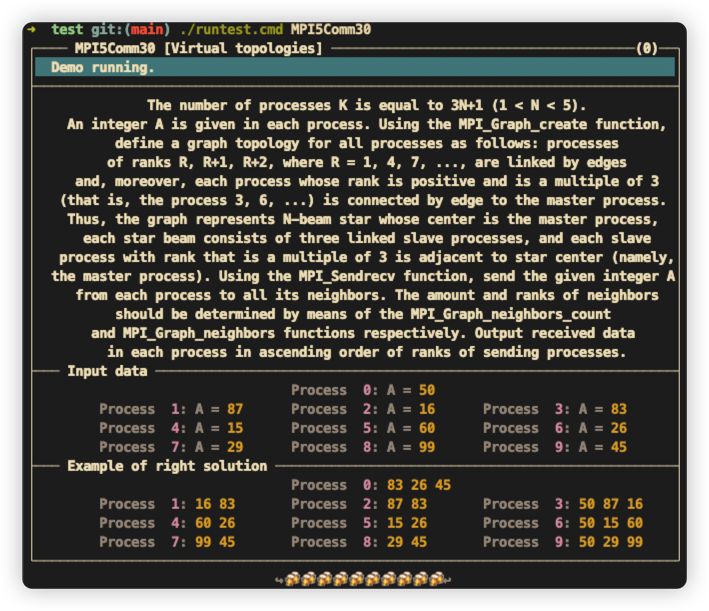
\includegraphics[width=0.65
    \linewidth]{images/example.jpg}%子图文件名
    \caption{demo info}%总标题
    \label{demo}%总标签
\end{figure}


\end{frame}
%---------------------------------------------------------

%---------------------------------------------------------

\begin{frame}{Ошибки компиляции}

\begin{figure}[htbp]%
    \centering
    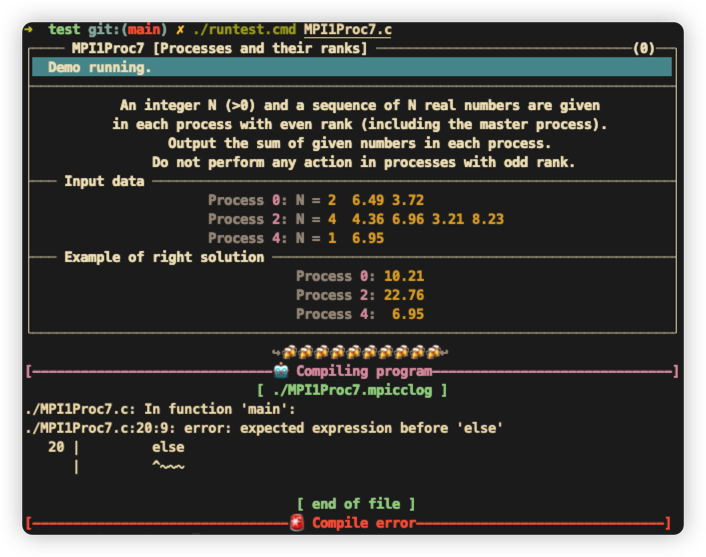
\includegraphics[width=0.65
    \linewidth]{images/error.jpg}%子图文件名
    \caption{error}%总标题
    \label{error}%总标签
\end{figure}
    
\end{frame}

%---------------------------------------------------------


%---------------------------------------------------------
%Two columns
\begin{frame}
\frametitle{MPI1Proc7}

\begin{columns}
\column{0.5\textwidth}
\begin{figure}[htbp]%
    \centering
    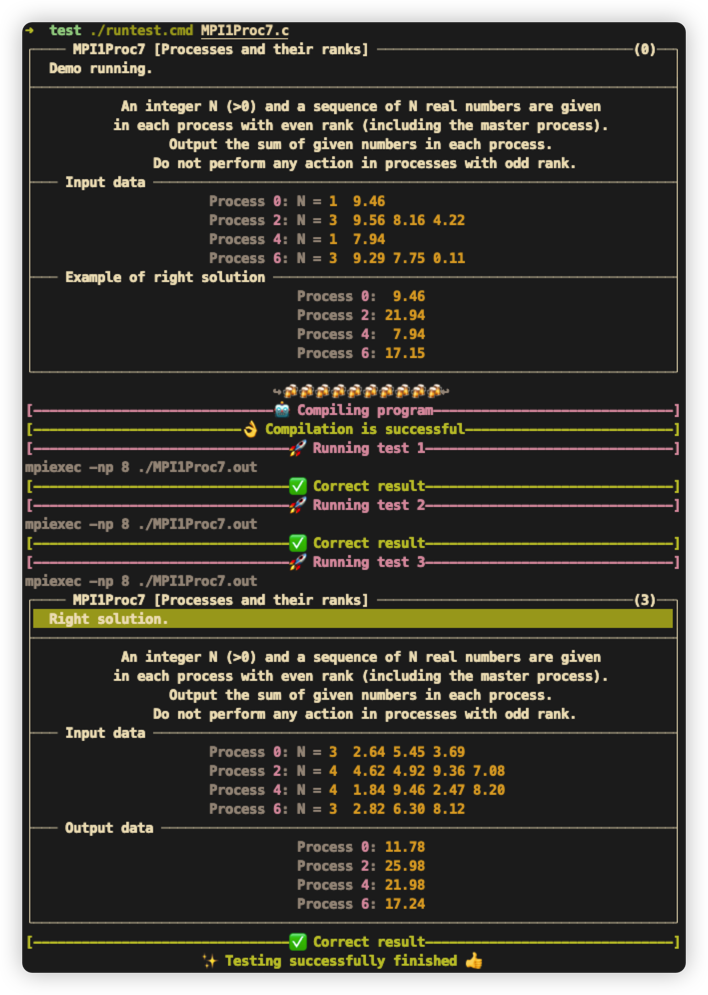
\includegraphics[width=0.77
    \linewidth]{images/mpi1_eg_r.jpg}%子图文件名
    \caption{right solution}%总标题
    \label{right}%总标签
\end{figure}
\column{0.5\textwidth}
\begin{figure}[htbp]%
    \centering
    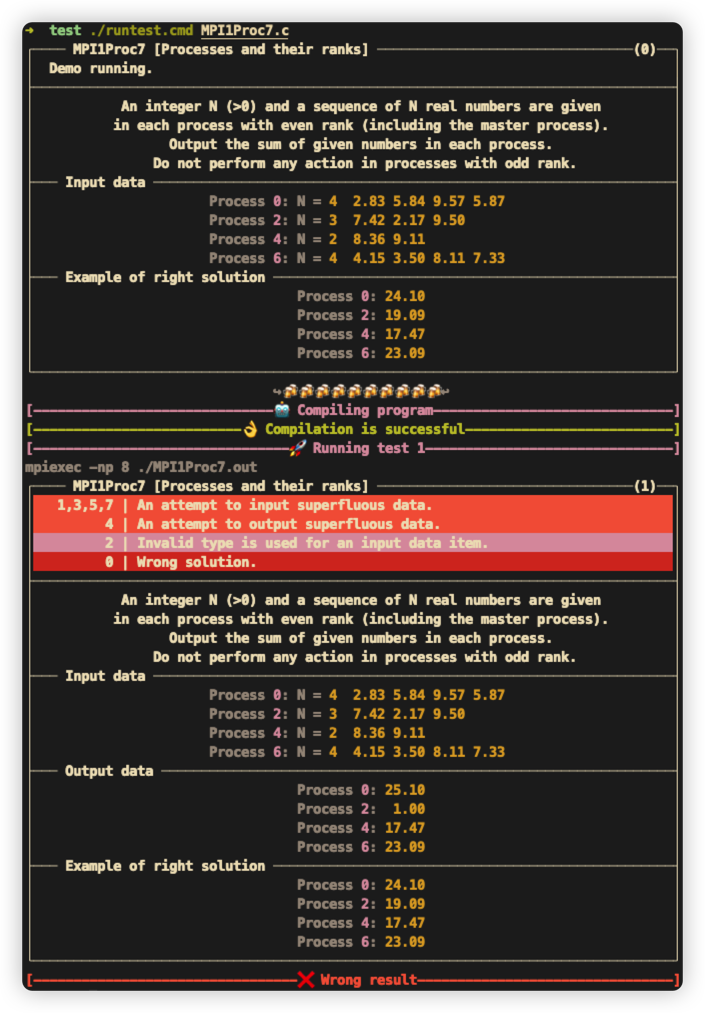
\includegraphics[width=0.75
    \linewidth]{images/mpi1_eg_w.jpg}%子图文件名
    \caption{wrong solution}%总标题
    \label{wrong}%总标签
\end{figure}

\end{columns}
\end{frame}
%---------------------------------------------------------